\pdfminorversion=4
\documentclass{beamer}
\usepackage[english]{babel}
\usefonttheme{professionalfonts} % using non standard fonts for beamer
\usefonttheme{serif} % default family is serif
\usetheme[hideothersubsections]{Hannover-perso}
\usecolortheme{crane-perso}

\def\swidth{1.6cm} \setbeamersize{sidebar width left=\swidth}

\logo{\includegraphics[height=.75 cm]{figures/AEM-prosper_no_bg}}

\setbeamertemplate{frametitle}[default][center]

\setbeamertemplate{sidebar left} { {
    \vskip1.5em%
    \hskip.1cm\insertlogo \vskip1.25em%
  }%
  {%
    \usebeamercolor[fg]{author in sidebar}%
    \usebeamerfont{author in sidebar}%
    \insertshortauthor[width=\swidth,center,respectlinebreaks]\par%
    \vskip3em%
  }%
  \vskip1.25em%
  \insertverticalnavigation{\swidth}%
  \vfill \hbox to2cm{\hskip0.6cm\usebeamerfont{section in
      sidebar}\strut\usebeamercolor[fg]{subsection in sidebar }
    \insertframenumber /\inserttotalframenumber }%
  \vskip3pt%
}%

\setbeamertemplate{headline}{}

\setbeamertemplate{navigation symbols}{}

\usepackage{color}
\usepackage{graphicx}
\usepackage{amsfonts}
\usepackage{mathrsfs}
\usepackage{soul}
\usepackage{bm}
\usepackage{algpseudocode}
\usepackage{algorithm}
\usepackage{textcomp}
\usepackage{listings}
\usepackage{stackengine}
\usepackage{amsmath}
\usepackage{environ}
\usepackage{xmpmulti}
\usepackage{animate}

\stackMath

\DeclareMathOperator{\diag}{diag}

\newcommand{\norm}[1]{\lVert#1\rVert}

\newcommand{\norma}[1]{\left\lVert#1\right\rVert}

\newcommand{\little}[1]{\scalebox{0.7}}

\NewEnviron{little_eq}{
	\begin{equation*}
    \scalebox{1.0}{$\BODY$}
    \end{equation*}
    }

\AtBeginSection[]{
	\begin{frame}
	%\vfill
	\vspace{0.5 in}
	\centering
	\usebeamerfont{section title}\insertsectionhead
	\end{frame}
}



%************************************************************
\begin{document}
\title{Stability and Bifurcations of a Non-Uniform Compressed Elastic Strip}%\\[1cm]}%
\author[A. J. Akerson]{Andrew J. Akerson\\[10pt]
  \footnotesize akers049@umn.edu}%
\date{Masters Exam, May 10, 2018}%
\institute{University of Minnesota, Minneapolis (MN), USA}%

\begin{frame}
  \titlepage
\end{frame}

\begin{frame}
  \frametitle{Outline}
  \tableofcontents[hideallsubsections]
\end{frame}

\section{Introduction}

\begin{frame}
	\frametitle{\large Introduction to Wrinkling and Surface Instabilities}
		\framesubtitle{Applications}
	Soft materials in compression \textrightarrow{} large deformation buckling.
	\begin{itemize}
	\item Biological systems
	\item Soft Actuators
	\item Electoric devices
	\end{itemize}
 	
 	\includegraphics[width=0.3\textwidth]{myFigures/biologicalThing}
	\includegraphics[width=0.3\textwidth]{myFigures/softActuator}
	\includegraphics[width=0.3\textwidth]{myFigures/bread}
	
		\scriptsize[\color{orange} Bo Li \textit{et. al.}(2012); Kostas \textit{et. al.} (2017); Hohlfeld \& Mahadevan (2011)\color{black}]

\end{frame}

\begin{frame}
	\frametitle{\large Introduction to Wrinkling and Surface Instabilities}	
	\begin{columns}
	\column{0.4\textwidth}
 	\scriptsize{Even simple 2-D Problems can have multiple equillibrium configurations:
	}
	\column{0.6\textwidth}
	\includegraphics[width = \textwidth]{myFigures/basic_bifs}
	\end{columns} 	
	\vspace{0.1in}
	
	We will look at a similar 2-D problem of finite thickness strip of infinite length in compression:
	
		\begin{center}	
		\includegraphics[scale=0.25]{myFigures/compressed_strip_drawing}
	\end{center}
	
	
	\scriptsize[\color{orange} Qiming Wang \& Xuanhe Zhao(2015))\color{black}]	
\end{frame}

\begin{frame}
	\frametitle {\large Related work}

	\begin{columns}
	\column {0.45 \textwidth} 	\begin{center}	Biot looked at compressed 2-D half-space in 1961.
		\includegraphics[scale=0.25]{myFigures/halfSpace}
	\end{center}
	\column {0.45 \textwidth}	
	\begin{center}
Further work on elastic half space:
	\includegraphics[scale=0.35]{myFigures/wrinklingPicture}
	\end{center}
	\end{columns}
	
	\vspace{0.1 in}
	\begin{center}
	Half-space that uses bloch-wave:
	\includegraphics[scale=0.7]{myFigures/bertoli}
	\end{center}
		
	\scriptsize[\color{orange} Biot (1961); Diab \textit{et. al.}(2013); Zhao \textit{et. al.} (2015), Liu \& Bertoli (2015) \color{black}]
\end{frame}

\begin{frame}
	\frametitle{\large Our Viewpoint}
	Things missing or unclear that we would like to address:
	\begin{itemize}
 
		\begin{columns}
				\column{0.35 \textwidth}
				\item Relations between instabilities through \color{blue} bifurcation diagram\color{black}.
				
				\column{0.5 \textwidth}	
				\begin{center}
			    \includegraphics[scale=0.4]{myFigures/simpleBifDiagram}					
				\end{center}

		
			  \end{columns} 

		
		\item Understand how problem parameters 
		
		(ie. film/substrate stiffness) effects these instabilities
		\item Analytical description of finite thickness problem.
	\end{itemize}		
	
\end{frame}

\section{Problem Statement}

\begin{frame}
	\frametitle{\large Problem Statement}
	Finite thickness, infinite length strip:
	\begin{center}	
		\includegraphics[scale=0.4]{myFigures/compressed_strip_drawing}
	\end{center}
	
	Displacement control: $\lambda = 1 - \lambda_1$
	
	2-D Compressible Plane Strain NeoHookean Constituitive:
	\begin{equation*} 
		W(\mathbf{F})=\mu(x_2)\left[\frac{1}{2}(I_1 - 2- \ln{I_2}) + \frac{\nu}{1-\nu}(\sqrt{I_2} - 	1)^2\right],
	\end{equation*}
	Where:	$\qquad I_1 = \mathrm{tr}\mathbf{C} \qquad I_2 = \mathrm{det} \mathbf{C} $	
	
	\vspace{0.05in}
	And use: $\nu = 0.33$
	
\end{frame}

\begin{frame}
	\frametitle{\large Problem Statement}
	
	Consider Two Cases:
	\begin{enumerate}
	\item  Exponential : $\mu(x_2) = \mu_0 e^{\kappa x_2}$
	\item  Piecewise Constant: $
\mu(x_2) = 
\left \{ 
\begin{aligned} 
  \mu &= \mu_1 \quad 0 \leq x_2 < L_1 \\
  \mu &= \mu_2 \quad L_1 \leq x_2 \leq L
\end{aligned} 
\right \}$

\begin{flushright}
Use $L_1/L = 0.9$. 
\end{flushright}


\vspace{0.1 in}
	\begin{center}
		\includegraphics[scale=0.4]{myFigures/compressed_strip_drawing_piece_const}
	\end{center}
	\end{enumerate}
	
\end{frame}

\section{First Bifurcation}

\begin{frame}
	\frametitle{\large Equillibrium}\begin{equation*}	
	\mbox{Total strain energy: } \mathcal{E}(\mathbf{u}, \lambda) = \int_\Omega W(\mathbf{F}) dA
\end{equation*}
	Equillibrium condition:
	\footnotesize 
	\begin{equation*}
	\mathcal{E},_{\mathbf{u}}(\mathbf{u}, \lambda) \delta\mathbf{u} = \int_\Omega  \frac{\partial W}{\partial {F_{ij}}} \delta F_{ij} \,dA = 0 \quad \forall \delta\mathbf{u} \in \mathcal{U}
	\end{equation*}
	\normalsize

\includegraphics[width = \textwidth]{myFigures/stability}
	
\end{frame}

\begin{frame}
\frametitle{\large Principal Solution}
Equillibrium solution that passes through $(\mathbf{u}, \lambda) = (\mathbf{0}, 0)$	.

Denote principal solution $\stackon{\mathbf{u}}{0}$
\begin{center}
	\includegraphics[width = 0.7\textwidth]{myFigures/principal}
\end{center}
	\begin{itemize}
	\item 	Assume uniform $\mathbf{F}_{0} = \diag[\lambda_1,\lambda_2]$
	\item First PK Stress: $\mathbf{\Pi} = \left . \frac{\partial W}{\partial \mathbf{F}} \right|_{\mathbf{F}_{0}} = \diag[\Pi_{11}, \Pi_{22}], $	
	\begin{center}
	\scriptsize{$\begin{aligned}
\Pi_{11} &= \mu(x_2) \left [ \lambda_1 - \lambda_1^{-1} + \frac{2\nu}{1 -\nu}(\lambda_1 \lambda_2^2 - \lambda_2) \right ] , \\
\Pi_{22} &= \mu(x_2) \left [ \lambda_2 - \lambda_2^{-1} + \frac{2\nu}{1 - \nu}(\lambda_1^2 \lambda_2 - \lambda_1) \right ]. 
\end{aligned} $}
\end{center}
	\item Enforcing the zero normal traction at $x_2 = L$:
	\footnotesize{	
	\begin{equation*}
  \Pi_{22} |_{x_2 = L} = 0  \quad \implies \quad \lambda_2 - \lambda_2^{-1} + \frac{2\nu}{1 - \nu}(\lambda_1^2 \lambda_2 - \lambda_1) = 0
	\end{equation*}}
\end{itemize}	 

Also required that $\stackon{\mathbf{u}}{0}$ is stable in neighborhood of $\lambda = 0$
\end{frame}

\begin{frame}
	\frametitle{\large Stability and First Bifurcation}
	
Second variation of energy: 
\footnotesize
\begin{equation*}
(\mathcal{E},_{\mathbf{u} \mathbf{u}}\delta\mathbf{u})\delta\hat{\mathbf{u}} = \int_\Omega  \frac{\partial^2 W}{\partial F_{ij} F_{kl}} \delta F_{ij} \delta \hat{F}_{kl} \,dA = \int_\Omega  \frac{\partial^2 W}{\partial F_{ij} F_{kl}} \delta u_{i,j} \delta \hat{u}_{k,l} \,dA
\end{equation*}
\normalsize
Stability Condition:
\begin{center}
$(\mathcal{E},_{\mathbf{u} \mathbf{u}}(\mathbf{u}, \lambda) \delta\mathbf{u}) \delta\mathbf{u} \geq \beta(\mathbf{u}, \lambda) \norma{\delta \mathbf{u}}^2, \quad \beta > 0$ 
\end{center}
Along Principle Solution:

\begin{itemize}
	\item Stable near $\lambda = 0$
	\item Stable up to $\lambda < \lambda_c$
	\item Unstable for $\lambda \geq \lambda_c$
\end{itemize}
$\implies$ Then at $\lambda_c$ : $(\mathcal{E},_{\mathbf{u} \mathbf{u}}(\stackon{\mathbf{u}}{0}, \lambda_c) \stackon{\mathbf{u}}{1}) \delta\mathbf{u} = 0 , \quad \norm{\stackon{\mathbf{u}}{1}}^2 = 1$
\end{frame}

\begin{frame}
\frametitle{\large First Bifurcation, continued}
Solve for exponential case:
\footnotesize
\begin{equation*}
(\mathcal{E},_{\mathbf{u} \mathbf{u}}(\stackon{\mathbf{u}}{0}, \lambda_c) \stackon{\mathbf{u}}{1}) \delta\mathbf{u} = \int_\Omega  \left. \frac{\partial^2 W}{\partial F_{ij} F_{kl}} \right |_{\lambda_c} \stackon{u}{1}_{i,j} \delta u_{k,l} \,dA = 0
\end{equation*}
\normalsize
IBP, div theorem, and sub $\left. \frac{\partial^2 W}{\partial F_{ij} F_{kl}} \right |_{\lambda_c} = L^c_{ijkl}(x_2)$ :  
\footnotesize
\begin{equation*}
- \int_{\Omega} \left ( L^c_{ijkl}(x_2) \: \stackon{u}{1}_{i,j} \right )_{,l} \: \delta u_k \: \,dA + \int_{\partial \Omega} L^c_{ijkl}(x_2) \: \stackon{u}{1}_{i,j} \: n_l \:  \delta u_k \: \,ds = 0
\end{equation*}
\normalsize
First expression gives a linear PDE for $\stackon{\mathbf{u}}{1}$ :
\footnotesize \begin{equation*}
 \left ( L^c_{ijkl}(x_2) \: \stackon{u}{1}_{i,j} \right )_{,l} = L^c_{ijkl,2}(x_2) \: \stackon{u}{1}_{i,j} +  L^c_{ijkl}(x_2)\stackon{u}{1}_{i,jl} = 0,  \quad k = 1,2
\end{equation*} \normalsize

Second gives the natural B.C's
\end{frame}

\begin{frame}
\frametitle{\large First Bifurcation, continued}
Recall: $\qquad \mu(x_2) = \mu_0 e^{\kappa x_2}, \qquad W(\mathbf{F}) = \mu(x_2) \tilde{W}(\mathbf{F})$
\vspace{0.1in}
So our PDE becomes:
\footnotesize \begin{equation*}
 \kappa \tilde{L}^c_{ijkl} \: \stackon{u}{1}_{i,j} +  \tilde{L}^c_{ijkl}\stackon{u}{1}_{i,jl} = 0,  \quad k = 1,2
\end{equation*} \normalsize
Constant coefficient (for a given $\lambda$) linear homogenous. Separation gives:

\scriptsize \begin{equation*} 
\left \{ 
\begin{aligned} 
  \stackon{u}{1}_1 &= -v_1(x_2)\sin(\omega x_1) \\
  \stackon{u}{1}_2 &=  v_2(x_2)\cos(\omega x_1)
\end{aligned} 
\right \}  \qquad 
\left \{ 
\begin{aligned} 
  \stackon{u}{1}_1 &= v_1(x_2)\cos(\omega x_1) - v_1(0) \\
  \stackon{u}{1}_2 &=  v_2(x_2)\sin(\omega x_1)
\end{aligned} 
\right \}
\end{equation*} 
\normalsize
\begin{equation*}
v_1(x_2) = \sum_{i = 1}^{4}A_ie^{\alpha_i x_2}, \qquad v_2(x_2) = \sum_{i = 1}^{4} A_i B_i e^{\alpha_i x_2}.
\end{equation*}  
\begin{itemize} 
	\item $\omega$ related to wavelength. $B_i$'s, and $\alpha$'s known.
	\item Only Unknowns are $A_i$'s
\end{itemize}
\end{frame}

\begin{frame}
\frametitle{\large First Bifurcation, continued}
Need to find when there exist $A_i$'s that satisfy the B.C's.
\begin{itemize}
	\item Plug our solution into 3 Natural B.C's \& $\stackon{u}{1}_2(x_1, 0) = 0$ 
	\begin{center}
	$\mathbf{M(\omega, \lambda)} \, \mathbf{A} = \mathbf{0}, \quad \mathbf{A} = [ A_1, A_2, A_3, A_4 ]^T$ \end{center}
	\item Solution exists when $\det(\mathbf{M}) = 0$
\end{itemize}



Our Procedure:
\begin{enumerate}
	\item Choose many $\omega$'s
	\item For each solve for the lowest $0 < \lambda_c < 1$ that satisfies $\det(\mathbf{M}) = 0$
	\item The wavelength associated with the smallest $\lambda_c$ is the first mode to go unstable.  
\end{enumerate}

\end{frame}

\begin{frame}
\frametitle{\large First Bifurcation Exponential Case}

\center{
		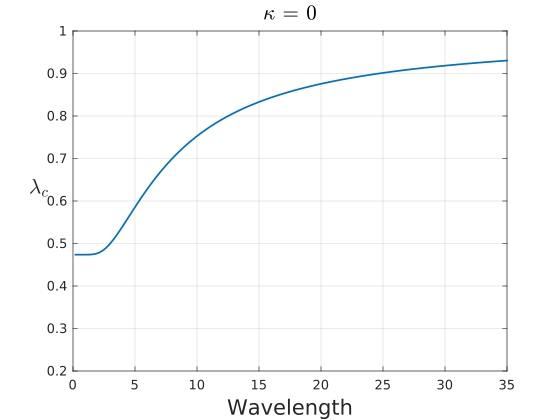
\includegraphics[width=0.45\textwidth]{myFigures/firstBif_lambdac_exp_0}
		}
		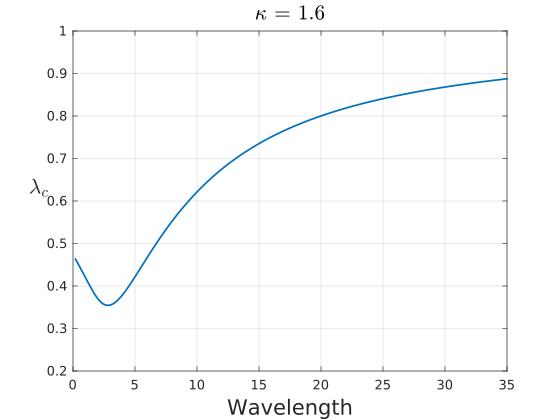
\includegraphics[width=0.45\textwidth]{myFigures/firstBif_lambdac_exp_1_6}	
		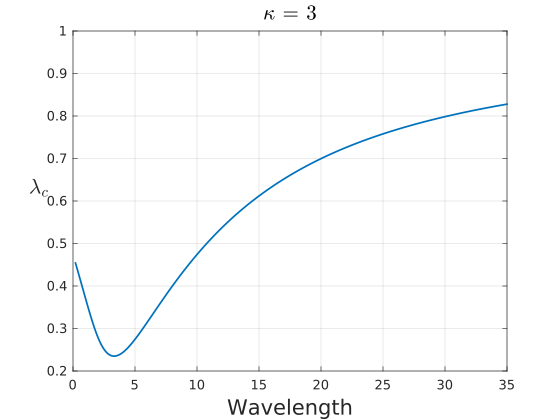
\includegraphics[width=0.45\textwidth]{myFigures/firstBif_lambdac_exp_3_0}


\end{frame}

\begin{frame}
\frametitle{\large First Bifurcation Piecewise Constant Case}
Similar procedure as exponential case.
\center{
		\includegraphics[width=0.45\textwidth]{myFigures/firstBif_lambdac_pieceConst_2}
		}
		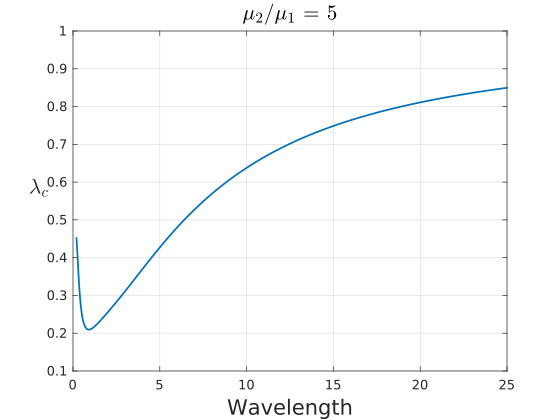
\includegraphics[width=0.45\textwidth]{myFigures/firstBif_lambdac_pieceConst_5}	
		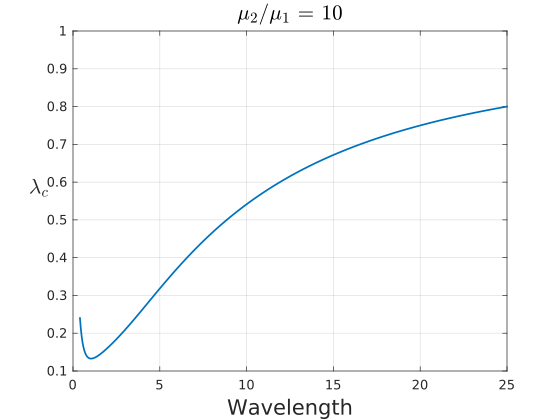
\includegraphics[width=0.45\textwidth]{myFigures/firstBif_lambdac_pieceConst_10}
\end{frame}

\section{FEM}
\begin{frame}
\frametitle{Finite Element Implementation}
Critical wavelength gives the unit cell length for simulation.
\begin{columns}
	\column{0.65 \textwidth}
		\begin{itemize}
		\item Discretize body
		\item Solution is interpolation of displacements at nodes
		\item Solve for when $\frac{\partial\mathcal{E}}{\partial \mathbf{u}} = \mathbf{R}(\mathbf{u}) =  \mathbf{0}$ by Newton-Rapson Iteration:
		\center{
		 $\frac{\partial^2\mathcal{E}}{\partial\mathbf{u}\partial\mathbf{u}} \Delta\mathbf{u}  = \mathbf{K}(\mathbf{u}_i)\Delta\mathbf{u}  =  -\mathbf{R}(\mathbf{u}_i) $
		 
		 $ \mathbf{u}_{i + 1} = \mathbf{u}_i + \Delta \mathbf{u}$
		}
		\end{itemize}
	\column{0.35 \textwidth}
		\center{
		\includegraphics[width = 0.7 \textwidth]{myFigures/undeformedMesh}
		}
\end{columns}
\vspace{0.1in}
Implimented in the C++ deal.ii finite element library. 
\begin{itemize}
	\item \color{blue} Matrices are accessable
	\item Takes care of: shape functions, mappings, mesh generation, linear solver
	\item \color{red} Write code to assemble matrices and do iterations
\end{itemize}

\end{frame}


\begin{frame}
\frametitle{\large Finite Element}
Standard FEM: Increment $\lambda$, Newton iterate, repeat.


Use Pseudo-Archlength Continuation approach:
\begin{columns}

\column{0.45 \textwidth}
\begin{itemize}
	\item Make $\lambda$ a DOF 
	\begin{center}
	$\tilde{\mathbf{u}}$ = 
	$\begin{bmatrix}
	  \mathbf{u} \\ 
	  \lambda 
	\end{bmatrix} $
	\end{center}
	\item Add constraint: \footnotesize $ ds = \sqrt{ \norm{\mathbf{u}_{i} - \mathbf{u}_{i - 1}}^2 + \Delta \lambda}$
	\normalsize	
\end{itemize}

\column{0.55 \textwidth}
\begin{center}
	 \includegraphics[width = \textwidth]{myFigures/PACA}
\end{center}
\end{columns}
\begin{itemize}
	\item Enforce by: \footnotesize
	$\tilde{\mathbf{R}}$ = 	
	$\begin{bmatrix}
	  \mathbf{R} \\ 
	  \frac{1}{2}(\norm{\mathbf{u}_{i} - \mathbf{u}_{i-1}}^2 + \Delta \lambda ^2 - ds^2)
	\end{bmatrix} $  = 
		$\begin{bmatrix}
	  \mathbf{R} \\ 
	  \eta
	\end{bmatrix} $ 
	\normalsize
	
	\item Then Newton iterate: $\tilde{\mathbf{K}}(\tilde{\mathbf{u}}_i) \Delta \tilde{\mathbf{u}} = -\tilde{\mathbf{R}}(\tilde{\mathbf{u}}_i)$
	\vspace{0.05 in}
	
	Where: $\tilde{\mathbf{K}}(\tilde{\mathbf{u}}) = $
	$\begin{bmatrix}
	  \mathbf{K}(\mathbf{u}) & \frac{\partial\mathbf{R}}{\partial \lambda} \\ 
	  \left[ \frac{\partial \eta}{\partial \mathbf{u}} \right]^T & \frac{\partial{\eta}}{\partial \lambda}
	\end{bmatrix} $ 
\end{itemize}
\end{frame}

\begin{frame}{Embedded Animation}
	\frametitle{FEM}
	
	Now we can follow our first bifurcated solution :
	
  \animategraphics[loop,controls,width= 0.90\linewidth]{20}{myFigures/deformation_animation/def_exp_3-}{0}{93}
%		    \transduration<0-16>{0}
%        \multiinclude[<+->][format=png, graphics={width=\textwidth}]{myFigures/deformation_animation/def_exp_3}
        
\end{frame}

\begin{frame}
	\frametitle{Stability}

	\begin{itemize}
		\item Stability from eigenvalues of $\mathbf{K}(\mathbf{u})$.
		\item But only gives info on the projected problem of critical wavelength periodicity.

	\end{itemize}
	
	\begin{center}
	\textbf{What if there exist further instabilities that are of different periodicity than the original unit cell length?}
	\end{center}
	\begin{center}
		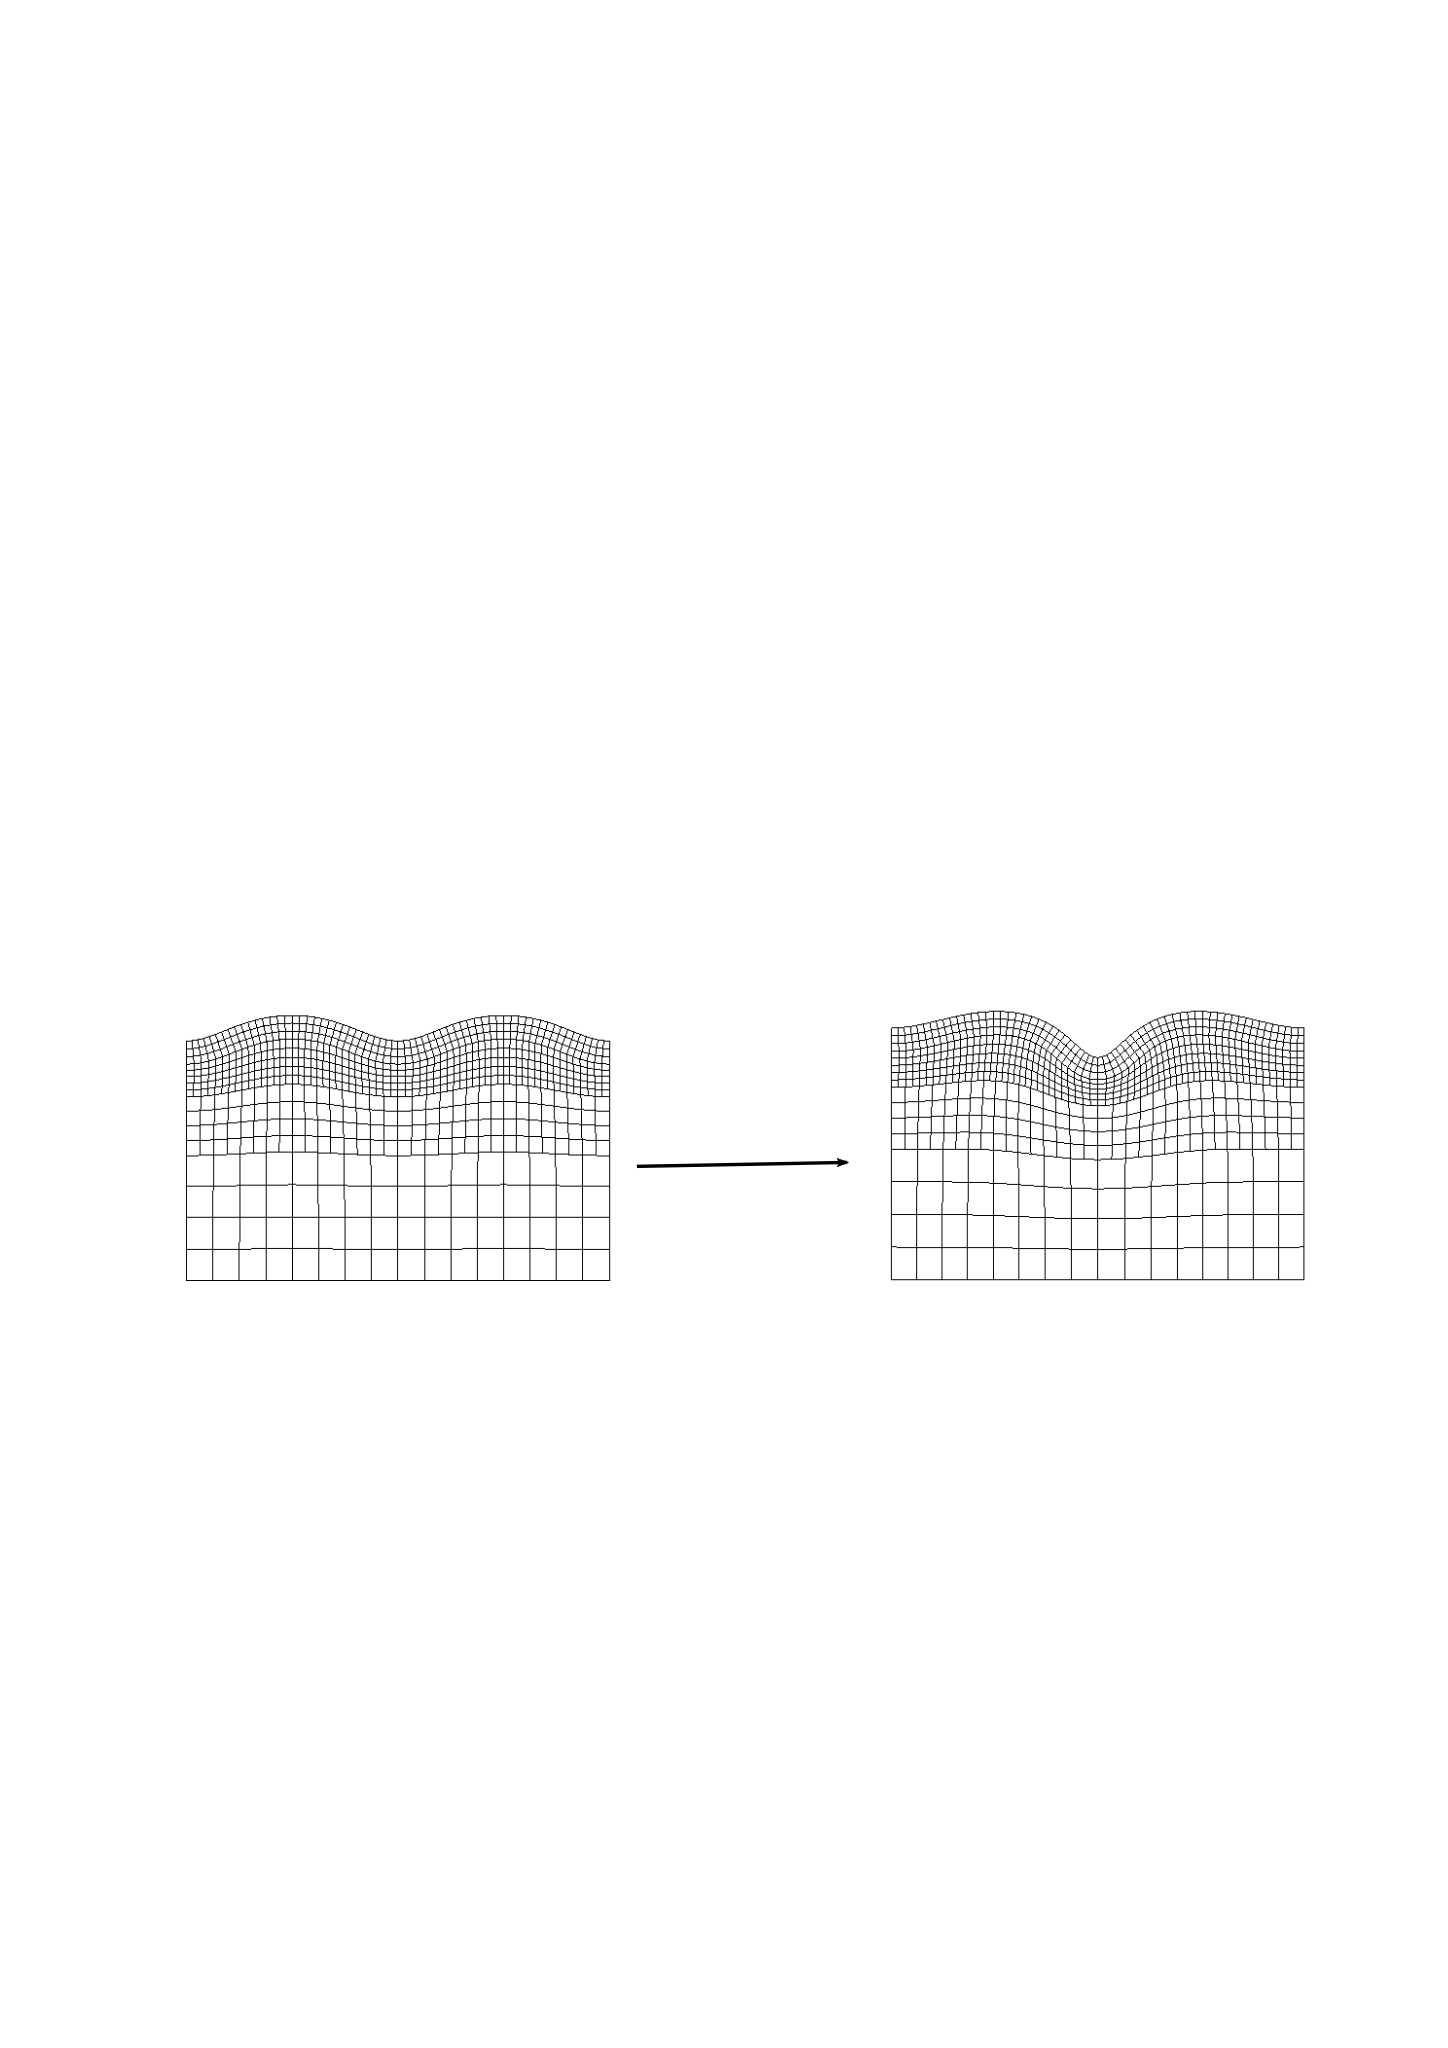
\includegraphics[width = 0.7\textwidth]{myFigures/periodic_change}
	\end{center}		
	
	\vspace{0.3 in}	
	We can investigate this with \color{blue}\textbf{Bloch Wave}  \color{black}B.C.'s.
	
	
\end{frame}

\section{Bloch Wave}

\begin{frame}

	\frametitle{Bloch Wave B.C.'s}
	\begin{center}
	\includegraphics[width = 0.5\textwidth]{myFigures/blochDiagram}
	\end{center}
	Apply Bloch Wave Boundary Conditions: 
	\begin{equation*}
		\mathbf{u}(x_1 + l_1, x_2) = \mathbf{u}(x_1, x_2) e^{i \omega l_1}, \quad \text{where}: \omega = \frac{2 \pi}{l_2}
	\end{equation*}
	\begin{itemize}
		\item 	Eigenvalues of resulting stiffness matrix gives stability info for modes of periodicity $l_2$
		\item Do for many $\omega$'s, get global stability info.	
	\end{itemize}
	
\end{frame}

\begin{frame}

	\frametitle{Bloch Wave B.C.'s, cont}
	\begin{columns}
		\column{0.3 \textwidth}
		Verification along principal:
		\column {0.6 \textwidth}
		\begin{center}
	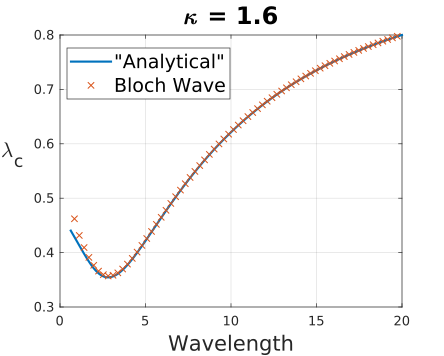
\includegraphics[width = 0.75\textwidth]{myFigures/blochWaveWorks}	
	\end{center}
	\end{columns}
	

	
		\footnotesize Typical Bloch wave results at a step
	\begin{columns}
		\column{0.42 \textwidth} \tiny \center{Stable}
			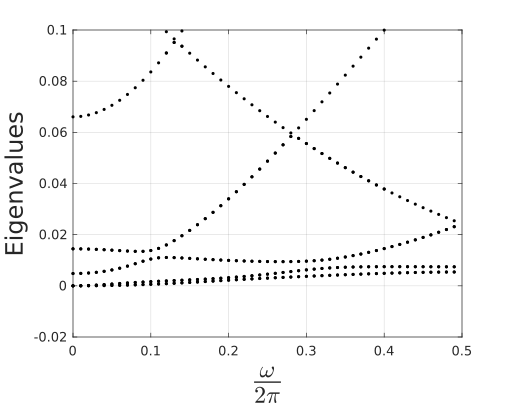
\includegraphics[width =\textwidth]{myFigures/blochWave_stable}
		\column{0.42 \textwidth} \tiny \center{Unstable} 
			\includegraphics[width =\textwidth]{myFigures/blochWave_unstable}

	\end{columns}
	\normalsize
\end{frame}	

\begin{frame}
	\frametitle{\large Procedure with Bloch Wave}
	
	\begin{enumerate}
		\item Follow first bifurcated path with periodic domain of length equal to critical wavelength.
		\item Every step compute bloch eigs for range of $\omega$.
		\item When a mode goes unstable, resize domain to that of unstable mode and begin following the new bifurcation.
		\begin{enumerate}[\color{red}(i)]
		
		\item Reinitialize a mesh with periodicity of unstable mode.
		\item Follow the same first bifurcated path,  now with the new periodicity.
		\item When eigenvalue of stiffness matrix $\mathbf{K}$ changes sign, follow the new unstable mode.
		\end{enumerate}

		\item Repeat steps (2) - (3) (if computationally feasible). 
	\end{enumerate}
\end{frame}


\begin{frame}
	\frametitle{\large Example Diagram}
	
	Now we can go ahead and follow some paths and make bifurcation diagrams:
	\begin{columns}
		\column{0.20 \textwidth}
			\color{red} 2 - periodic
			
			\color{blue} 3 - periodic
			
		\column{0.8 \textwidth}
		\begin{center}
			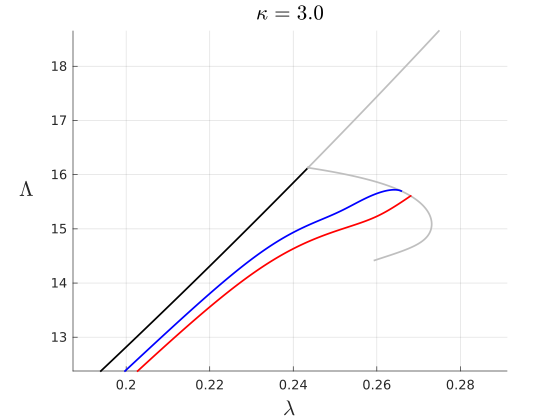
\includegraphics[width = 0.9\textwidth]{myFigures/bif_diagram_exp_3_0}
		\end{center}	
	\end{columns}

\vspace{0.05 in}	
	\color{black}
	Congugate loading parameter: $\Lambda \equiv \dfrac{d\mathcal{E}}{d\lambda}$
\end{frame}

\begin{frame}
	\frametitle{Some Problems}
	
	But this brings up some challenges:
	\begin{itemize}
		\item \color{red} These runs are computationally expensive.
		\item Sometimes tedious setting step size and other run parameters to get good results.
		\item To get full understanding, would need to run for a range of system parameters (ie. $\kappa$, $\mu_2/\mu_1$.).
	\end{itemize}
	\vspace{0.15 in}
	
	Would like to know the stability information of first bifurcated path ahead of time. 
	\vspace{0.15 in}	
	
	 Would allow us to smartly choose as few runs to still get full range of the problem.
	
\end{frame}

\section{Asymptotics}
\begin{frame}
	\frametitle{\large LSK Theory}
	Do this by Lyapunov - Schmidt - Koiter (LSK) Asymptotics.
	
	\vspace{0.15 in}
	Bifurcation amplitude parameter: 
	\begin{center}
		$ \xi \equiv (\mathbf{u} - \stackon{\mathbf{u}}{0}(\lambda_c), \stackon{\mathbf{u}}{1})$ 
	\end{center}
	
	Decompose: $\mathbf{u} = \stackon{\mathbf{u}}{0}(\lambda_c) + \xi \stackon{\mathbf{u}}{1} + \mathbf{v}, \quad $  
	where $(\mathbf{v},  \stackon{\mathbf{u}}{1}) = 0$ 
	
	$\mathbf{v}$ can be written as an expansion about $(\xi, \Delta \lambda) = (0,0)$ :
	\begin{center}
		$\mathbf{v} = \xi \mathbf{v}_{\xi} + \Delta \lambda \mathbf{v}_{\lambda} + \frac{1}{2}[\xi^2\mathbf{v}_{\xi \xi} + 2\xi \Delta\lambda \mathbf{v}_{\lambda \xi} + \Delta \lambda^2 \mathbf{v}_{\lambda \lambda}] + \ldots $
	\end{center}		
	
	Taylor expand $\Delta \lambda$:
	\begin{center}
		$ \Delta \lambda = \lambda_1 \xi + \frac{1}{2} \lambda_2 \xi^2 + \mathcal{O}(\xi^3) =  \frac{1}{2} \lambda_2 \xi^2 + \mathcal{O}(\xi^3) \quad \text{(for sym bif)}$ 
	\end{center}
	\vspace{0.05in}
	\center \scriptsize[\color{orange} Triantafyllidis \& Peek (1995) \color{black}]
\end{frame}

\begin{frame}
	\frametitle{\large LSK Theory, continued}
	
	Plug all of the relations from the previoius slide into the equillibrium equations,
	\footnotesize
	\begin{align*}
		\mathcal{E},_{\mathbf{v}}\delta \mathbf{v} = 0 \implies \mathcal{E},_{\mathbf{u}}(\stackon{\mathbf{u}}{0}(\lambda_c) + \xi \stackon{\mathbf{u}}{1} + \mathbf{v}, \lambda_c + \Delta \lambda) \delta \mathbf{v} &= 0 \\
		\mathcal{E},_{\xi} = 0 \implies \mathcal{E},_{\mathbf{u}}(\stackon{\mathbf{u}}{0}(\lambda_c) + \xi \stackon{\mathbf{u}}{1} + \mathbf{v}, \lambda_c + \Delta \lambda) \delta \stackon{\mathbf{u}}{1} &= 0
	\end{align*}		
	\normalsize
	Get the following relations (among other things):
	\footnotesize
	\begin{center}
		$(\mathcal{E}^c,_{\mathbf{u} \mathbf{u}} \mathbf{v}_{\xi \xi} + (\mathcal{E}^c_{\mathbf{u} \mathbf{u} \mathbf{u}} \stackon{\mathbf{u}}{1}) \stackon{\mathbf{u}}{1} ) \delta \mathbf{v} = 0 $
		\vspace{0.2 in}
		
		
		$ \lambda_2 = -\frac{1}{3} \frac{(((\mathcal{E}^c_{\mathbf{u} \mathbf{u} \mathbf{u} \mathbf{u}} \stackon{\mathbf{u}}{1}) \stackon{\mathbf{u}}{1}) \stackon{\mathbf{u}}{1}) \stackon{\mathbf{u}}{1} 
		+ 3 ((\mathcal{E}^c,_{\mathbf{u} \mathbf{u} \mathbf{u}} \mathbf{v}_{\xi \xi})\stackon{\mathbf{u}}{1})\stackon{\mathbf{u}}{1}}{((d\mathcal{E}^c,_{\mathbf{u} \mathbf{u}}/d\lambda)\stackon{\mathbf{u}}{1})\stackon{\mathbf{u}}{1}}$
	\end{center}
	\normalsize
	Solve for $\mathbf{v}_{\xi \xi}$ in the first one, then plug into second to get $\lambda_2$
	
	\vspace{0.1in}
	\center \scriptsize[\color{orange} Triantafyllidis \& Peek (1995) \color{black}]

\end{frame}

\begin{frame}
	\frametitle{\large Soliving for $\mathbf{v}_{\xi \xi}$ }
	\footnotesize	
	\begin{equation*}
		(\mathcal{E}^c,_{\mathbf{u} \mathbf{u}} \mathbf{v}_{\xi \xi} + (\mathcal{E}^c_{\mathbf{u} \mathbf{u} \mathbf{u}} \stackon{\mathbf{u}}{1}) \stackon{\mathbf{u}}{1} ) \delta \mathbf{v} = 0 
	\end{equation*}
	\normalsize
	Solve similar to first bifurcated mode:
	\tiny
\begin{multline*}
\int_{\partial \Omega} \left[ L^c_{ijkl}(x_2) \: v_{\xi \xi i,j} +  M^c_{ijklmn} \stackon{u}{1}_{m,n} \stackon{u}{1}_{i,j} \right] n_l \delta v_{k} ds \\
- \int_{\Omega} \left[ \left( L^c_{ijkl}(x_2) \: v_{\xi \xi i,j} \right)_{,l} \: + \left(M^c_{ijklmn} \stackon{u}{1}_{m,n} \stackon{u}{1}_{i,j} \right )_{,l} \right ] \delta v_k \: \,dA = 0 
\end{multline*}
\normalsize
This gives us a linear, inhomogenous, PDE and B.C's. 
		
Using known $\stackon{\mathbf{u}}{1}$ and $M^c_{ijklmn}$, find our solution is of the form:
\begin{center}
	$v_{\xi \xi_1}  = g_1(x_2) \sin(2 \omega_c x_1) \qquad v_{\xi \xi_2}  = g_2(x_2) \cos(2 \omega_c x_1) + \tilde{g}_2(x_2)$
\end{center}
\begin{itemize}
	\item $g_1(x_2)$ and $g_2(x_2)$ satisfy an inhomogenous $\text{2}^{\text{nd}}$ order system of ODE's.
	\item $\tilde{g}_2(x_2)$ satisfies an inhomogenous $\text{1}^{\text{st}}$ order ODE.
\end{itemize}

\underline{Solve these semi-analytically.}
\end{frame}

\begin{frame}
	\frametitle{\large LSK for $\Lambda$ }
	
	Now that we have $\mathbf{v}_{\xi \xi}$ we can easily solve for $\lambda_2$.
	
	\vspace{0.1 in}
	
	Can expand congugate loading parameter at bif.\ point:
	\begin{center}
		$ \Delta \Lambda = \Lambda_1 \xi + \frac{1}{2} \Lambda_2 \xi^2 + \mathcal{O}(\xi^3) =  \frac{1}{2} \Lambda_2 \xi^2 + \mathcal{O}(\xi^3) \quad \text{(for sym bif.)}$ 
	\end{center}
	
	From taking derivatives of $\Lambda$ with $\xi$, we find:
	\footnotesize
	\begin{equation*}
	 \Lambda_2 = ((d\mathcal{E}^c,_{\mathbf{u} \mathbf{u}}/d\lambda)\stackon{\mathbf{u}}{1})\stackon{\mathbf{u}}{1} + (d\mathcal{E}^c,_{\mathbf{u}}/d\lambda) \mathbf{v}_{\xi \xi} + \lambda_2(d\mathcal{E}^c,_{\mathbf{u}}/d\lambda) \frac{\partial \stackon{\mathbf{u}}{0}}{\partial \lambda}
	\end{equation*}
	\normalsize
	
	\textbf{With $\lambda_2$ and $\Lambda_2$ we have behavior near bif.\ point.}
	\begin{enumerate}
		\item Choose a many parameter values (either $\kappa$ or $\frac{\mu_2}{\mu_1}$)
		\item For each, solve for $\mathbf{v}_{\xi \xi}$
		\item Use this to compute $\lambda_2$, then $\Lambda_2$.
	\end{enumerate}		
	
\end{frame}

\begin{frame}
	\frametitle{\large Verify $\lambda_2$ and $\Lambda_2$ correct}
	\begin{columns}
		\column{0.2 \textwidth} \footnotesize \center Exponential
		\column{0.45 \textwidth}
		\center \includegraphics[width =\textwidth]{myFigures/lambdaCheck_exp_1}
		
		\column{0.45 \textwidth}
				\center \includegraphics[width = \textwidth]{myFigures/lambdaCheck_exp_2}
	\end{columns}

	\begin{columns}
		\column{0.2 \textwidth} \footnotesize \center Piecewise Constant
	
		\column{0.45 \textwidth}
		\center \includegraphics[width = \textwidth]{myFigures/lambdaCheck_pieceConst_1}
		
		\column{0.45 \textwidth}
				\center \includegraphics[width = \textwidth]{myFigures/lambdaCheck_pieceConst_2}
	\end{columns}
	
	
\end{frame}

\begin{frame}
	\frametitle{Exponential}
	
	\includegraphics[width = \textwidth]{myFigures/lambdas_exp}
\end{frame}

\begin{frame}
	\frametitle{Piecewise Constant}
	\includegraphics[width = \textwidth]{myFigures/lambdas_pieceConst}
\end{frame}

\section{Bifurcation Diagrams}

\begin{frame}
	\frametitle {Piecewise Constant Bifurcation Diagrams}
	
	\begin{columns}
		\column{0.5 \textwidth}
			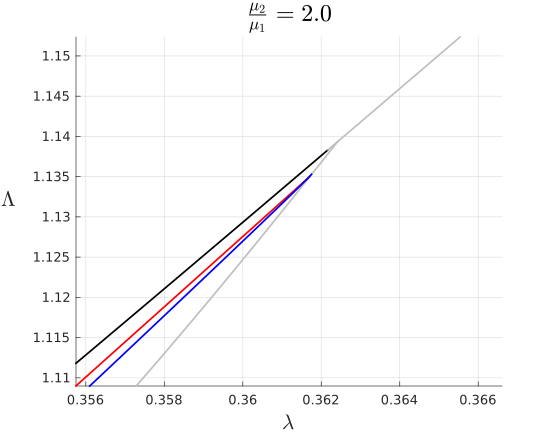
\includegraphics[ width = \textwidth]{myFigures/bif_diagram_20}
		\column{0.5 \textwidth}
			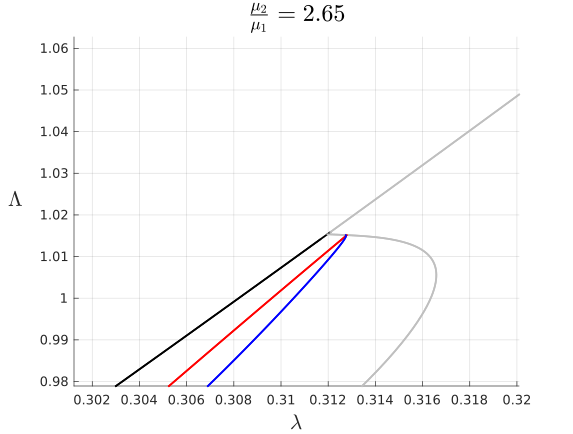
\includegraphics[ width = \textwidth]{myFigures/bif_diagram_265}
	\end{columns}
	\begin{columns}
		\column{0.2 \textwidth}
			\vspace{0.1 in}
			
	\color{red} 2-periodic 
	
	\color{blue} 3-periodic
		\column{0.8 \textwidth}
		\flushright{
		\includegraphics[width = 0.6\textwidth]{myFigures/lambdas_pieceConst}}
		
	\end{columns}

\end{frame}

\begin{frame}
	\frametitle{$ \mu_2 / \mu_1 = 10$}
	\begin{center}
	\includegraphics[width = 0.6\textwidth]{myFigures/slice1}
	\end{center}
	\color{red} 2-periodic 
	
	\color{blue} 3-periodic
\end{frame}

\begin{frame}
	\frametitle{$ \mu_2 / \mu_1 = 10$}
	\begin{center}
	\includegraphics[width = 0.6\textwidth]{myFigures/slice2}
	\end{center}
	\color{red} 2-periodic 
	
	\color{blue} 3-periodic
\end{frame}

\begin{frame}
	\frametitle{$ \mu_2 / \mu_1 = 10$}
	\begin{center}
	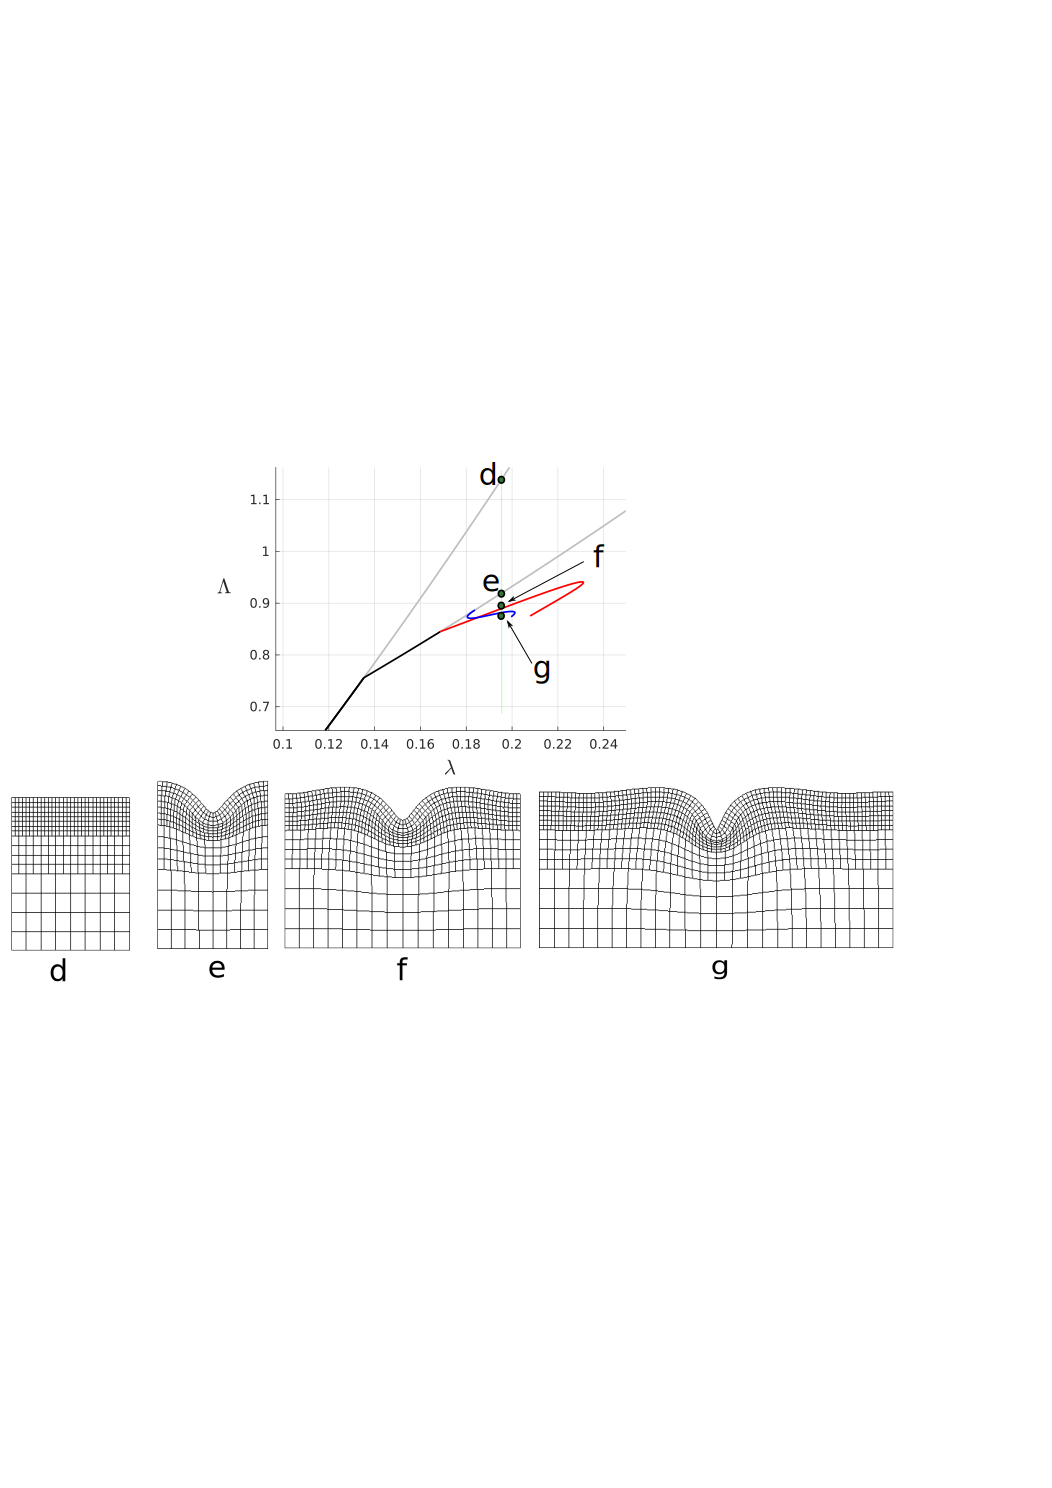
\includegraphics[width = \textwidth]{myFigures/slice3}
	\end{center}
	
	\color{red} 2-periodic 
	
	\color{blue} 3-periodic
\end{frame}

\section{Summary}

\begin{frame}
	\frametitle{What We Have Done}
	\begin{itemize}
		\item Solved for critical load and wavelength of first bifurcation (semi-analytically).
		
		\item Wrote FEM code with equillibrium path following to follow the bifurcated branch.
		
		\item Incorporated Bloch Wave to the FEM code to study stability and further bifurcations of different periodicity.
		
		\item Carried out asymptotic calculations for understanding stability and path properties at initial bifurcation point.
		
		\item Allows us to wisely select cases to run the code on.
	\end{itemize}

\end{frame}

\begin{frame}
	\frametitle{What is Next?}
	Immidiately:
	\begin{itemize}
		\item Run some more verification on asymptotics.
		
		\item Spend some time making code more robust.

	\end{itemize}
	
	More Broadly:
	
	\begin{itemize}
		\item Run Bloch Wave on secondary bifurcations 
		
		(look for further bifurcations).
		
		\item Mesh refinement study and explore some of the 
		turning point behavior. 
		
		\item Explore how other factors affect wrinkling (magenetoelastic film with applied magnetic field)
	\end{itemize}
\end{frame}

\begin{frame}
\begin{center}
	\huge \textbf{Thanks!}
	
	\includegraphics[width = \textwidth]{myFigures/bunanddino}
\end{center}

\end{frame}


\end{document}
